\documentclass[10pt,a4paper]{article}
\usepackage[utf8]{inputenc}
\usepackage{amsmath}
\usepackage{amsfonts}
\usepackage{amssymb}
\usepackage{graphicx, xcolor, threeparttable, booktabs, tikz}
\usepackage[a4paper,text={16.5cm,25.2cm},centering]{geometry}
\usepackage{bm}
\parindent=0pt

\usepackage[style=authoryear-comp, backend=bibtex, natbib=true]{biblatex}
\bibliography{WickEtAl2018}

\begin{document}
\today
\section*{Author response to reviewers}
We would like to thank both the referees for their valuable comments and positive feedback on our paper. We have now thoroughly revised our paper to address your comments. We believe that this has resulted in a much-improved paper. We hope that you agree. Please find below our responses to your comments (in {\color{blue} blue} font).

\subsection*{Author responses to comments by reviewer 1}
\begin{enumerate}
	\item Forecast combinations with non-negative weights, for example applied to disaggregate forecasts to compute an aggregate forecasts, share similar problems with forecast reconciliation. The major difference is probably that weights in forecast reconciliations do not sum to one as they do in forecast combinations. It will be worth to make this clear and {\color{red} explain what this implies in terms of computational time.}
	\item [] {\color{blue} Forecast reconciliation has some similarities with forecast combinations, but with the following differences: (1) the combination weights are partially determined by the aggregation structure of the time series; (2) we only produce one forecast for each series; (3) the forecast of each series is a combination of the forecasts of all series; (4) the forecast weights are not restricted to add to 1 or to be non-negative. Typically, in forecast combination problems, the combination weights are free to be selected or estimated by the user, there are multiple forecasts for each series, the final forecast of each series is a combination only of forecasts for that series, and the forecast weights are normally restricted to be non-negative and to sum to one.

  We have now added this paragraph at the end of Section 2.1.

  While the problems share some similarities, the differences noted above make any direct comparisons of computational time largely meaningless.

	% We can illustrate the forecast reconciliation process considering the simplest hierarchy involving one level of disaggregation with two series at the bottom level i.e., $y_{Z, t} = y_{X, t} + y_{Y, t}$ with the following covariance matrix of the $h$-steps ahead base forecast errors:
	% \begin{align*}
	% \bm{W}_h = \begin{bmatrix}
	% \sigma^2_{Z, h} & \sigma_{XZ, h} & \sigma_{YZ, h}\\
	% \sigma_{XZ, h} & \sigma^2_{X, h} & \sigma^2_{XY, h}\\
	% \sigma_{YZ, h} & \sigma_{XY, h} & \sigma^2_{Y, h}
	% \end{bmatrix}.
	% \end{align*}


	% Table~\ref{tbl:reconpros} compares the reconciliation process on each of the bottom-level base forecasts for different choices of $\bm{\Lambda}_h$.

	% \begin{table}[ht]
	% 	\caption{Reconciliation process of the bottom-level base forecasts.}
	% 	\label{tbl:reconpros}
	% 	\centering
	% 	\begin{threeparttable}
	% 		\begin{tabular}{lcl}
	% 			\toprule
	% 			Approach & $\bm{\Lambda}_h = $ & Reconciliation process\\
	% 			\midrule
	% 			MinT & $\bm{W}_{h}$ & $\displaystyle \hat{y}_{X, T}(h) + \frac{\sigma_{X, h}^{2} + \sigma_{XY, h} - \sigma_{XZ, h}}{\sigma_{h}^{2}}\bigtriangleup_{h}$\\[0.4cm]
	% 			& & $ \displaystyle \hat{y}_{Y, T}(h) + \frac{\sigma^{2}_{Y, h} + \sigma_{XY, h} - \sigma_{YZ, h}}{\sigma_{h}^{2}}\bigtriangleup_{h}$\\[0.4cm]
	% 			WLS & $\text{diag}(\bm{W}_h)$ & $\displaystyle\hat{y}_{X, T}(h) + \frac{\sigma^{2}_{X, h}}{\sigma^{2}_{Z, h} + \sigma^{2}_{X, h} + \sigma^{2}_{Y, h}}\bigtriangleup_{h}$\\[0.4cm]
	% 			& & $\displaystyle \hat{y}_{Y, T}(h) + \frac{\sigma^{2}_{Y, h}}{\sigma^{2}_{Z, h} + \sigma^{2}_{X, h} + \sigma^{2}_{Y, h}}\bigtriangleup_{h}$\\[0.4cm]
	% 			OLS & $\sigma^2\bm{I}; \sigma^2 > 0$ & $\displaystyle \hat{y}_{X, T}(h) + \frac{1}{3}\bigtriangleup_{h}$\\[0.4cm]
	% 			& & $\displaystyle \hat{y}_{Y, T}(h) + \frac{1}{3}\bigtriangleup_{h}$\\
	% 			\midrule
	% 			\multicolumn{2}{l}{\text{where:}}\\[0.4cm]
	% 			\multicolumn{2}{c}{$\displaystyle \bigtriangleup_{h} = \hat{y}_{Z, T}(h) - [\hat{y}_{X, T}(h) + \hat{y}_{Y, T}(h)]$}\\[0.4cm]
	% 			\multicolumn{2}{c}{$\displaystyle \sigma_{h}^{2} = \sigma^{2}_{Z, h} - 2\sigma_{XZ, h} - 2\sigma_{YZ, h} + \sigma^{2}_{X, h} + \sigma^{2}_{Y, h} + 2\sigma_{XY, h}$}\\
	% 			\bottomrule
	% 		\end{tabular}
	% 		\begin{tablenotes}
	% 			\item [] Notes: $\bigtriangleup_{h}$ measures the magnitude of incoherence of the bottom-level base forecasts, whereas $\sigma_{h}^{2}$ in the denominator of MinT can be written equivalently as $\text{Var}\{\hat{e}_{Z, T}(h) - [\hat{e}_{X, T}(h) + \hat{e}_{Y, T}(h)]\}$, with $\hat{e}_{Z, T}(h)$, $\hat{e}_{X, T}(h)$ and $\hat{e}_{Y, T}(h)$ being the $h$-step-ahead base forecast errors of the total, $X$ and $Y$ series, respectively.
	% 		\end{tablenotes}
	% 	\end{threeparttable}
	% \end{table}
	% For MinT, the numerator for series $X$ measures the difference between $\text{Cov}[\hat{e}_{Z, T}(h), \hat{e}_{X, T}(h)]$ and $\text{Cov}[\hat{e}_{X, T}(h) + \hat{e}_{Y, T}(h), \hat{e}_{X, T}(h)]$, which should ideally be zero if the base forecasts are themselves coherent. Thus, it adjusts the series more if the incoherence is large. Similarly, WLS places a higher weight on $\bigtriangleup_{h}$ for the series with higher base forecast error variances. These results are as we would expect, as series with higher incoherence should require more amendments. However, OLS assigns the same weight to $\bigtriangleup_{h}$ for both series, which is not very intuitive.
	}

	\item The new method adds an important step to the MinT approach. However, forecast gains are almost negligible in simulation and empirical exercises. Even OLS produce accurate forecasts. Why is this the case? I will work out an exercise where optimal non-negative forecast reconciliation gives large gains otherwise the reader will be confused on the utility of the new method.
	\item [] {\color{blue} The purpose of non-negative forecast reconciliation is not necessarily to improve forecast accuracy but to align the forecasts with their use in practice. Many forecasts are of inherently non-negative variables such as sales volume or expenditure. In such cases, it is important to users that the forecasts are also non-negative. In cases where forecasts are provided at several levels of aggregation, it is also important that the forecasts are coherent. If forcing non-negative coherence on the forecasts improves accuracy, it is a side benefit, not the main purpose.

  In any case, Table 7 does not reflect forecast gains through reconciliation. It only shows the percentage relative improvement of non-negative reconciled forecasts over the same reconciliation method without the non-negativity constraints. Hence, we cannot expect large gains in forecast accuracy to be seen in this table.

	The forecasting performance results for each of these non-negative reconciliation approaches are given in Table~\ref{tbl:rmsenn}. Each negative (positive) entry shows the percentage (decrease) increase in average RMSEs relative to the base forecasts. The top panel shows the results using the ARIMA base forecasts, while the bottom panel shows the results using the ETS base forecasts. It is clear immediately from both panels that minT(Shrink) is the best performing forecast reconciliation approach. The WLS$_v$ and OLS also perform well, generally showing improvements over the base forecasts.

	\begin{table*}[!htb]
		\centering
		\fontsize{9}{12}\rm\tabcolsep=0.095cm
		\caption{Out-of-sample forecast performances for Australian domestic tourism flows.}
		\label{tbl:rmsenn}
		\begin{threeparttable}
			\begin{tabular}{lrrrrrrrrrrrrrrr}
				\toprule
				& \it{$h=1$} & \it{2} & \it{3} & \it{6} & \it{12} & \it{1--6} & \it{1--12} &  & \it{$h=1$} & \it{2} & \it{3} & \it{6} & \it{12} & \it{1--6} & \it{1--12} \\
				\cline{2-8} \cline{10-16} \\[-0.3cm]
				& \multicolumn{15}{c}{ARIMA} \\
				\cline{2-16} \\[-0.3cm]
				& \multicolumn{7}{c}{Australia} & & \multicolumn{7}{c}{Australia by purpose of travel} \\
				\cline{2-8}\cline{10-16} \\[-0.3cm]
				OLS & $-3.5$ & $-2.2$ & $-2.7$ & $-2.4$ & $-2.9$ & $-2.9$ & $-2.8$ & & $-0.4$ & $-1.4$ & $-0.7$ & $-1.8$ & $-1.8$ & $-0.9$ & $-0.9$ \\
				WLS$_v$ & $-0.6$ & 1.5 & $-0.1$ & 0.2 & $-4.2$ & $-0.6$ & $-0.9$ & & 4.8 & 3.7 & 3.5 & 2.4 & 1.0 & 3.4 & 3.0 \\
				MinT & $\bf{ -8.0}$ & ${\bf -5.9}$ & ${\bf -8.0}$ & ${\bm -6.2}$ & ${\bf -8.5}$ & ${\bf -7.5}$ & ${\bf -7.2}$ & & ${\bf -5.0}$ & ${\bf -5.5}$ & ${\bf -6.4}$ & ${\bf -6.4}$ & ${\bf -6.2}$ & ${\bf -5.9}$ & ${\bf -5.6}$ \\
				\cline{2-8}\cline{10-16} \\[-0.3cm]
				& \multicolumn{7}{c}{States} & & \multicolumn{7}{c}{States by purpose of travel} \\
				\cline{2-8}\cline{10-16} \\[-0.3cm]
				OLS & 0.8 & 0.2 & 0.5 & $-0.6$ & 1.2 & 0.3 & $-0.1$ & & 1.6 & 0.9 & 0.9 & 1.5 & 1.9 & 1.3 & 1.6 \\
				WLS$_v$ & $-0.1$ & $-0.3$ & 0.2 & $-0.9$ & $-1.1$ & $-0.4$ & $-0.8$ & & $-0.3$ & $-1.3$ & $-1.2$ & $-0.4$ & $-1.1$ & $-0.9$ & $-0.8$ \\
				MinT & ${\bf -5.2}$ & ${\bf -5.6}$ & ${\bf -5.4}$ & ${\bf -5.6}$ & ${\bf -4.5}$ & ${\bf -5.4}$ & ${\bf -5.5}$ & & ${\bf -4.4}$ & ${\bf -5.1}$ & ${\bf -5.4}$ & ${\bf -4.2}$ & ${\bf -4.1}$ & ${\bf -4.8}$ & ${\bf -4.5}$ \\
				\cline{2-8}\cline{10-16} \\[-0.3cm]
				& \multicolumn{7}{c}{Zones} & & \multicolumn{7}{c}{Zones by purpose of travel} \\
				\cline{2-8}\cline{10-16} \\[-0.3cm]
				OLS & $-3.8$ & $-3.9$ & $-3.3$ & $-3.5$ & $-2.4$ & $-3.5$ & $-3.2$ & & 0.8 & 0.6 & 0.6 & 0.5 & 1.2 & 0.7 & 0.7 \\
				WLS$_v$ & $-6.4$ & $-6.2$ & $-5.5$ & $-5.6$ & $-5.6$ & $-5.7$ & $-5.6$ & & $-2.6$ & $-2.7$ & $-2.6$ & $-2.5$ & $-2.5$ & $-2.6$ & $-2.6$ \\
				MinT & $\bf{ -8.5}$ & $\bf{ -8.7}$ & $\bf{ -8.0}$ & $\bf{ -7.7}$ & $\bf{ -7.0}$ & $\bf{ -8.0}$ & $\bf{ -7.7}$ & & $\bf{ -4.4}$ & $\bf{ -4.4}$ & $\bf{ -4.5}$ & $\bf{ -4.1}$ & $\bf{ -3.7}$ & $\bf{ -4.3}$ & $\bf{ -4.2}$ \\
				& \multicolumn{7}{c}{Regions} & & \multicolumn{7}{c}{Regions by purpose of travel} \\
				\cline{2-8}\cline{10-16} \\[-0.3cm]
				OLS & $-2.8$ & $-2.4$ & $-2.5$ & $-2.5$ & $-1.8$ & $-2.4$ & $-2.2$ & & $-0.1$ & 0.2 & 0.3 & 0.0 & 0.5 & 0.2 & 0.2 \\
				WLS$_v$ & $-5.4$ & $-5.0$ & $-4.7$ & $-4.5$ & $-4.6$ & $-4.8$ & $-4.6$ & & $-3.4$ & $-3.2$ & $-3.0$ & $-3.0$ & $-2.8$ & $-3.1$ & $-3.1$ \\
				MinT & $\bf{ -7.2}$ & $\bf{ -6.6}$ & $\bf{ -6.5}$ & $\bf{ -5.9}$ & $\bf{ -5.8}$ & $\bf{ -6.4}$ & $\bf{ -6.2}$ & & $\bf{ -4.6}$ & $\bf{ -4.3}$ & $\bf{ -4.1}$ & $\bf{ -3.9}$ & $\bf{ -3.7}$ & $\bf{ -4.2}$ & $\bf{ -4.1}$ \\
				\cline{2-8}\cline{10-16} \\[-0.3cm]
				& \multicolumn{15}{c}{ETS} \\
				\cline{2-16} \\[-0.3cm]
				& \multicolumn{7}{c}{Australia} & & \multicolumn{7}{c}{Australia by purpose of travel} \\
				\cline{2-8}\cline{10-16} \\[-0.3cm]
				OLS & $-2.0$ & $-2.0$ & $-2.5$ & $-2.3$ & $-2.9$ & $-2.3$ & $-2.3$ & & 0.9 & 0.6 & 1.7 & 1.4 & 0.8 & 1.4 & 1.1 \\
				WLS$_v$ & $-3.8$ & $-2.8$ & $-3.6$ & $\bf{ -3.4}$ & $\bf{ -5.0}$ & $-3.9$ & $-3.3$ & & $-0.5$ & $-0.1$ & 0.8 & 0.8 & $-1.5$ & 0.5 & 0.4 \\
				MinT & $\bf{ -4.2}$ & $\bf{ -3.3}$ & $\bf{ -4.1}$ & $\bf{ -3.4}$ & $-4.9$ & $\bf{ -4.1}$ & $\bf{ -3.6}$ & & $\bf{ -1.0}$ & $\bf{ -0.5}$ & \bf{ 0.4} & \bf{ 0.6} & $\bf{ -1.8}$ & \bf{ 0.2} & \bf{ 0.0} \\
				\cline{2-8}\cline{10-16} \\[-0.3cm]
				& \multicolumn{7}{c}{States} &  & \multicolumn{7}{c}{States by purpose of travel} \\
				\cline{2-8}\cline{10-16} \\[-0.3cm]
				OLS & 1.3 & 1.5 & 1.6 & 2.0 & 2.3 & 1.6 & 1.6 & & 0.3 & 0.6 & 0.7 & 0.4 & 1.3 & 0.5 & 0.6 \\
				WLS$_v$ & $-2.1$ & $-0.9$ & $-1.0$ & $\bf{ -0.4}$ & $-1.8$ & $-1.3$ & $-1.1$ & & $-2.1$ & $-1.5$ & $-1.4$ & $-1.8$ & $-2.1$ & $-1.8$ & $-1.8$ \\
				MinT & $\bf{ -2.3}$ & $\bf{ -1.1}$ & $\bf{ -1.2}$ & $\bf{ -0.4}$ & $\bf{ -1.9}$ & $\bf{ -1.4}$ & $\bf{ -1.3}$ & & $\bf{ -2.3}$ & $\bf{ -1.6}$ & $\bf{ -1.5}$ & $\bf{ -1.9}$ & $\bf{ -2.3}$ & $\bf{ -1.9}$ & $\bf{ -1.9}$ \\
				\cline{2-8}\cline{10-16} \\[-0.3cm]
				& \multicolumn{7}{c}{Zones} & & \multicolumn{7}{c}{Zones by purpose of travel} \\
				\cline{2-8}\cline{10-16} \\[-0.3cm]
				OLS & 0.8 & 0.3 & 0.6 & 0.8 & 1.5 & 0.7 & 0.7 & & 0.9 & 0.7 & 0.6 & 0.8 & 1.4 & 0.8 & 0.8 \\
				WLS$_v$ & $\bf{ -0.8}$ & $\bf{ -1.0}$ & $\bf{ -0.8}$ & $-0.3$ & $-0.5$ & $-0.6$ & $-0.6$ & & $-0.5$ & $-0.5$ & $-0.7$ & $-0.6$ & $-0.3$ & $-0.6$ & $-0.5$ \\
				MinT & $\bf{ -0.8}$ & $\bf{ -1.0}$ & $\bf{ -0.8}$ & $\bf{ -0.4}$ & $\bf{ -0.8}$ & $\bf{ -0.7}$ & $\bf{ -0.8}$ & & $\bf{ -0.6}$ & $\bf{ -0.7}$ & $\bf{ -0.8}$ & $\bf{ -0.7}$ & $\bf{ -0.6}$ & $\bf{ -0.7}$ & $\bf{ -0.8}$ \\
				\cline{2-8}\cline{10-16} \\[-0.3cm]
				& \multicolumn{7}{c}{Regions} & & \multicolumn{7}{c}{Regions by purpose of travel} \\
				\cline{2-8}\cline{10-16} \\[-0.3cm]
				OLS  & 0.1 & $-0.3$ & $-0.3$ & $-0.4$ & 0.0 & $-0.2$ & $-0.2$ & & 0.5 & 0.5 & 0.5 & 0.5 & 0.9 & 0.5 & 0.5\\
				WLS$_v$ & $-1.0$ & $\bf{ -1.2}$ & $-1.2$ & $\bf{ -1.2}$ & $-1.5$ & $-1.1$ & $-1.2$ & & $-0.6$ & $-0.5$ & $-0.5$ & $-0.6$ & $-0.4$ & $-0.5$ & $-0.5$ \\
				MinT & $\bf{ -1.1}$ & $\bf{ -1.2}$ & $\bf{ -1.3}$ & $\bf{ -1.2}$ & $\bf{ -1.7}$ & $\bf{ -1.2}$ & $\bf{ -1.3}$ & & $\bf{ -0.8}$ & $\bf{ -0.7}$ & $\bf{ -0.7}$ & $\bf{ -0.8}$ & $\bf{ -0.7}$ & $\bf{ -0.8}$ & $\bf{ -0.8}$ \\
				\bottomrule
			\end{tabular}
			\begin{tablenotes}
				\item [] Notes: A negative (positive) entry shows the percentage decrease (increase) in average RMSEs relative to the base reconciled forecasts. Bold entries identify the best performing approaches.
			\end{tablenotes}
		\end{threeparttable}
	\end{table*}

	This information has now been added to ???}

\end{enumerate}
\clearpage

\subsection*{Author responses to comments by reviewer 2}

\begin{enumerate}
\item The abstract is too long and does not get to the point in a concise way, please reformulate.
\item []{\color{blue}
	The sum of forecasts of disaggregated time series are often required to equal the forecast of the aggregate, giving a set of coherent forecasts. The least squares solution for finding coherent forecasts uses a reconciliation approach known as MinT, proposed by \citet{Wick2018}. The MinT approach and its variants do not guarantee that the coherent forecasts are non-negative, even when all of the original forecasts are non-negative in nature. This has become a serious issue in applications that are inherently non-negative such as with sales data or tourism numbers. While overcoming this difficulty, we reconsider the least squares minimization problem with non-negativity constraints to ensure that the coherent forecasts are strictly non-negative.

	The constrained quadratic programming problem is solved using three algorithms. They are the block principal pivoting (BPV) algorithm, projected conjugate gradient (PCG) algorithm, and scaled gradient projection (SGP) algorithm. A Monte Carlo simulation is performed to evaluate the computational performances of these algorithms as the number of time series increases. The results demonstrate that the BPV algorithm clearly outperforms the rest, and PCG is the second best. The superior performance of the BPV algorithm can be partially attributed to the alternative representation of the weight matrix in the MinT approach.

	An empirical investigation is carried out to assess the impact of imposing non-negativity constraints on forecast reconciliation. It is observed that slight gains in forecast accuracy have occurred at the most disaggregated level. At the aggregated level slight losses are also observed. Although the gains or losses are negligible, the procedure plays an important role in decision and policy implementation processes.}
\item The matrix $\bm{C}$ after eq (2) is not defined.
\item [] Consider the 2-level structure given in Figure~\ref{fig:hier2}. In this example, $m = 7, n = 4$, $\bm{y}_t = \left[y_t, y_{A, t}, y_{B, t}, y_{AA, t}, y_{AB, t}, y_{BA, t}, y_{BB, t}\right]^\top$ and
$$\bm{S} = \begin{bmatrix}
1 & 1 & 1 & 1\\
1 & 1 & 0 & 0\\
0 & 0 & 1 & 1\\
1 & 0 & 0 & 0\\
0 & 1 & 0 & 0\\
0 & 0 & 1 & 0\\
0 & 0 & 0 & 1
\end{bmatrix}$$
\begin{figure}[!htb]  \center
	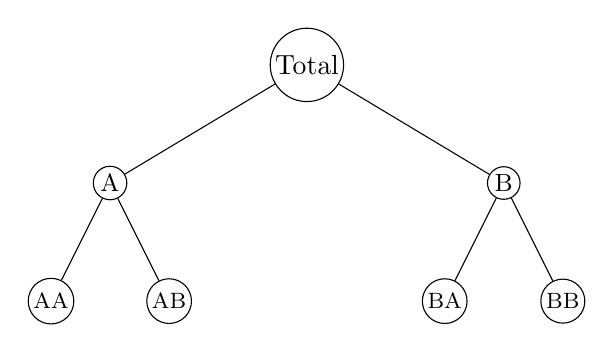
\begin{tikzpicture}
	\tikzstyle{every node}=[circle,draw,inner sep=1pt]
	\tikzstyle[level distance=.1cm]
	\tikzstyle[sibling distance=.1cm]
	%\tikzstyle{level 3}=[sibling distance=6.2mm,font=\tiny]
	\tikzstyle{level 1}=[sibling distance=50mm,font=\small]
	\tikzstyle{level 2}=[sibling distance=15mm,font=\footnotesize]
	\node{Total}%[edge from parent fork down]
	child {node {A}
		child {node {AA}}
		child {node {AB}}
	}
	child {node {B}
		child {node {BA}}
		child {node {BB}}
	};
	\end{tikzpicture}
	\caption{A two-level tree diagram.}
	\label{fig:hier2}
\end{figure}

{\color{red} We can include this on page 2, just after the first paragraph on Section 2.1.}

\item Non-negative least squares is not new can you provide references since the beginning?

\item [] {\color{blue} Yes, we agree that non-negative least squares is not a new field. We have mentioned on Page 3 that this area started with the work of Lawson and Hanson (1974) and have included a good reference (Chen and Plemmons (2009)) for a detailed review of this area. Therefore, we believe that a further review of non-negative least squares seems not relevant for this paper.}
\item \begin{enumerate}
	\item Assuming that $\bm{\Lambda}_h$ is positive definite does not seem so straightforward, that means that forecast errors are linearly independent, but if variables are highly collinear this might not happen. I think it all depends on how you compute $\hat{\bm{y}}_t(h)$. If forecast capture all comovements than I can believe the assumption. Some more explanation should be given.
	\item [] {\color{blue} Yes, the assumption of positive definiteness depends on how we compute $\hat{\bm{y}}_t(h)$. Unless we use very simple forecasting methods such as (seasonal) naive or linear trend models, it is very unlikely that the covariance matrix of the base forecast errors is positive semi-definite.}

	{\color{red} We can write a sentence on page 3 around line 41.}
	\item I see you compute univariate forecasts (via ARMA) but why not using multivariate methods in high-dimensions, e.g. factor models (see Stock and Watson, 2002), this would control better $\bm{\Lambda}_h$.

	\item [] {\color{blue} There are many multivariate models, such as factor models, VARMA, multivariate state space models, etc. Theoretically, we can expect these models to perform better than univariate models. However, the number of unknown parameters to be estimated is huge for a large structure. The estimation can also be prohibitive if there are insufficient number of observations. Even with a reasonable number of observations, the computing algorithms can be extremely slow.\\

	One of the main reasons for reconciliation is to avoid multivariate forecasting. We do univariate forecasts for each series, and then the relationships between the series are captured by estimating the covariance matrix of base forecast errors. It would largely defeat the purpose and simplicity of our approach to add multivariate forecasting.}
\end{enumerate}
\item ``large size of the structures that typically arise if forecast reconciliation" what are the orders of magnitude? Your application has 555 series which can be handled by multivariate forecasting methods.
\item [] {\color{blue} Please refer to the previous comment about multivariate forecasting models. One of the authors of this paper has applied reconciliation to around 1 million series in an industry project based in UK.}
\item When you define $\bm{\lambda}^*$ that is equal the derivative of $q$ wrt $\bm{b}$ while you are writing the opposite fix the notation.
\item [] {\color{blue} Thanks for pointing this, now we have corrected it in the revised document.}
\item Why in (9) you use the norm to define a quadratic loss? Keep the same notation as before.
\item [] {\color{blue} We have corrected this in the revised document.}
\item \begin{enumerate}
	\item Given the computational cost of running a constrained minimization with respect to the unconstrained case, what would happen if once we compute (1) we just throw away the negative forecasts and compute $\tilde{\bm{y}}$ with the remaining ones?
	\item [] {\color{blue} If we throw away the negative reconciled forecasts from unconstrained minimization and compute $\tilde{\bm{y}}$ with the remaining, then it will not provide any guarantee that the elements of $\tilde{\bm{y}}$ are non-negative. Your suggestion is similar to the first iteration of the block principal pivoting algorithm if $\bm{\Lambda}_h$ is diagonal. However, the block principal pivoting algorithm deletes and add variables until it reaches the convergence - similar to stepwise regression.}
	\item Are we really after all $m$ forecasts? Can you provide more motivation?
	\item [] {\color{blue} Yes, we are interested in all $m$ forecasts. Generating accurate forecasts for each of the 555 time series within the Australian tourism grouping structure is imperative for the planning purposes of National, State and Local tourism authorities. Ensuring that these forecasts are reconciled across all geographical disaggregation levels and purposes of travel lead to coherent decision making across the various levels of management.}
	\item And anyway what happens if you just impose the negative forecast to be zero. Can you repeat Table 7 in this case? Still the numbers there do not seem dramatically large.
	\item [] {\color{blue} If we set the negative reconciled forecasts to zero without performing any NNLS algorithms will lead to a set of incoherent forecasts.}
\end{enumerate}
\item What is an ETS model?
\item [] {\color{blue} ETS is a class of state space models, and stands for Error, Trend, and Seasonality. We have now defined the acronym on page 9.}
\item You say you log-transform data to compute forecasts and then you back-transform but doesn't this amount to taking an exponential and therefore you must get positive values? This part should be clarified.
\item [] {\color{blue} Yes, the base forecasts are positive because of the exponentials. However, this back-transformation does not make the reconciled forecasts to be non-negative. Therefore, NNLS algorithms are important.}
\end{enumerate}
\end{document}